\chapter{Конформные отображения и предписание для рассеяния открытых струн}

\lectureoverview{Конформное отображение сначала возникает как практическая симметрия двумерной электростатики. Комплексная дифференцируемость делает эту симметрию вычислимой: уравнения Коши--Римана влекут уравнение Лапласа, а не зависящая от направления комплексная производная сохраняет углы. Имея в руках этот аппарат, мировую поверхность струны можно изображать в виде полосы, полуплоскости, цилиндра или диска, не изменяя физики. Тогда рассеяние открытых струн сводится к гауссову интегралу по траекториям на диске с вставками импульса на его границе, за которым следует интеграл по их неэквивалентным положениям.}

\section{Электростатика в двумерном мире}

Начнём с буквально двумерной электростатической задачи. Заряды и их силовые линии ограничены плоскостью; это не просто обычные трёхмерные заряды, движение которых случайно происходит в плоскости. Тогда закон Гаусса даёт
\begin{equation}
  F(r)\propto \frac{1}{r},
  \qquad
  V(r)\propto \log r,
  \label{eq:l08-two-dimensional-coulomb}
\end{equation}
поскольку поток проходит через окружность, длина которой растёт как \(r\).

Представим поле через скалярный потенциал \(\phi\). В соглашении о знаке, использованном на доске,
\begin{equation}
  \mathbf E=\nabla\phi,
  \qquad
  \nabla\cdot\mathbf E=\rho,
\end{equation}
и потому
\begin{equation}
  \nabla^2\phi
  =\frac{\partial^2\phi}{\partial x^2}
  +\frac{\partial^2\phi}{\partial y^2}
  =\rho.
  \label{eq:l08-poisson}
\end{equation}
В области без зарядов это сводится к уравнению Лапласа,
\begin{equation}
  \nabla^2\phi=0.
  \label{eq:l08-laplace-phi}
\end{equation}
\editorialnote{Во многих учебниках по электродинамике вводят
\(\mathbf E=-\nabla\Phi\), и тогда после поглощения констант получается
\(\nabla^2\Phi=-\rho\). В лекции используется противоположный знак потенциала. Уравнение без источников и все конформные рассуждения остаются неизменными.}

\begin{figure}[H]
  \centering
  \includegraphics[width=0.72\textwidth]{lecture_08_figure_01.png}
  \caption{Электростатические уравнения, записанные в виде двумерного оператора Пуассона.}
  \lectureframe{00:03:48}
  \label{fig:l08-electrostatics-board}
\end{figure}

Знак плюс между двумя пространственными производными существен. Он делает это уравнение эллиптическим, а не волновым. Конформные преобразования сохраняют его форму без источников, так что решение в одной области можно перенести в область другой формы вместе с граничными условиями. Это полезно в электростатике, двумерном течении жидкости и картографии ещё до того, как становится полезным в теории струн.

\begin{classroomqa}
\audiencequestion{Если лапласиан обращается в нуль, является ли это уравнением стоячей волны? \lecturetimestamp{00:05:35}}
\lecturerresponse{Нет. Обе пространственные производные имеют один и тот же знак, и производной по времени здесь нет. Для волнового уравнения требуется зависимость от времени с лоренцевым относительным знаком. Электростатика статична именно потому, что ничто, включая волну, не эволюционирует.}
\end{classroomqa}

\begin{classroomqa}
\audiencequestion{Есть ли ротор в двух измерениях?
\lecturetimestamp{00:06:06}}
\lecturerresponse{Да, но у него есть только одна независимая компонента. Для
\(\mathbf E=(E_x,E_y)\),
\[
  \operatorname{curl}_{2d}\mathbf E
  =\partial_yE_x-\partial_xE_y.
\]
Его можно представлять как компоненту, перпендикулярную доске, хотя внутренне двумерный мир не нуждается ни в каком внешнем перпендикулярном направлении. В более высоких измерениях соответствующий объект естественно является антисимметричной 2-формой.}
\end{classroomqa}

\section{Производная без предпочтительного направления}

Введём комплексные координаты на исходной плоскости и плоскости образа:
\begin{equation}
  z=x+iy,
  \qquad
  w=u+iv,
  \qquad
  w=w(z).
  \label{eq:l08-complex-coordinates}
\end{equation}
Здесь \(x,y,u,v\) вещественны. Локально производная должна быть
\begin{equation}
  \frac{dw}{dz}
  =\lim_{\Delta z\to0}\frac{\Delta w}{\Delta z}.
  \label{eq:l08-complex-derivative}
\end{equation}
Комплексная плоскость, в отличие от вещественной прямой, допускает бесконечно много направлений приближения. Непрерывное и в обычном смысле гладкое отображение не обязано давать одно и то же отношение вдоль каждого направления.

Сравним два простых способа подхода. По направлению \(x\), \(dy=0\), так что
\begin{equation}
  \left.\frac{dw}{dz}\right|_x
  =\frac{\partial u}{\partial x}
  +i\frac{\partial v}{\partial x}.
\end{equation}
По направлению \(y\), \(dx=0\), и
\begin{equation}
  \left.\frac{dw}{dz}\right|_y
  =\frac{1}{i}\frac{\partial u}{\partial y}
  +\frac{\partial v}{\partial y}
  =\frac{\partial v}{\partial y}
  -i\frac{\partial u}{\partial y}.
\end{equation}
Равенство действительной и мнимой частей даёт
\begin{equation}
  \boxed{
  \frac{\partial u}{\partial x}
  =\frac{\partial v}{\partial y},
  \qquad
  \frac{\partial u}{\partial y}
  =-\frac{\partial v}{\partial x}}
  \label{eq:l08-cauchy-riemann}
\end{equation}
Это уравнения Коши--Римана. При обычных предположениях дифференцируемости они также достаточны для того, чтобы предел
\eqref{eq:l08-complex-derivative} не зависел от направления. Функция с этим свойством аналитична, или голоморфна, в данной точке.

\begin{figure}[H]
  \centering
  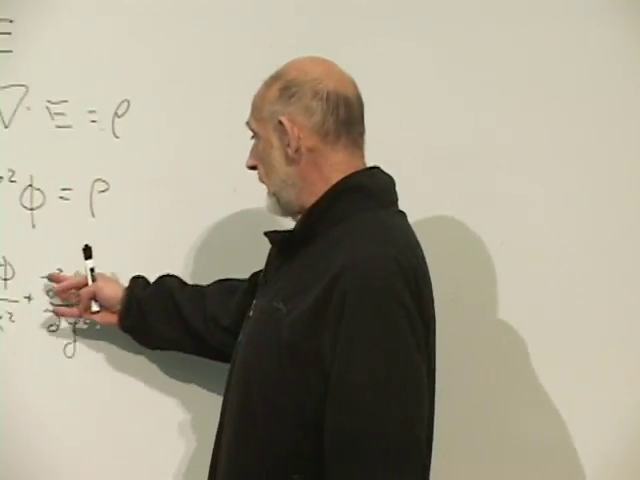
\includegraphics[width=0.70\textwidth]{lecture_08_figure_02.png}
  \caption{Полная пара уравнений Коши--Римана, включая относительный знак минус.}
  \lectureframe{00:19:48}
  \label{fig:l08-cr-board}
\end{figure}

В лекции кратко различается родственная терминология. Функция, голоморфная на всей конечной комплексной плоскости, называется целой. Мероморфная функция может иметь изолированные полюса. Поэтому \(1/z\) аналитична вне \(z=0\), но не является целой.

\section{Гармонически сопряжённые функции и конформная геометрия}

Уравнения Коши--Римана — это связанные уравнения первого порядка, но из них следуют отдельные уравнения второго порядка. Продифференцируем
\(\partial_xu=\partial_yv\) по \(x\), продифференцируем
\(\partial_yu=-\partial_xv\) по \(y\) и сложим:
\begin{align}
  \partial_x^2u&=\partial_x\partial_yv,\\
  \partial_y^2u&=-\partial_y\partial_xv,\\
  \therefore\qquad
  \partial_x^2u+\partial_y^2u&=0.
  \label{eq:l08-harmonic-u}
\end{align}
Повторение этого рассуждения с перестановкой \(u\) и \(v\) даёт
\begin{equation}
  \partial_x^2v+\partial_y^2v=0.
  \label{eq:l08-harmonic-v}
\end{equation}
Вещественная и мнимая части аналитической функции поэтому являются гармонически сопряжёнными. Две произвольные гармонические функции не образуют автоматически аналитическую функцию; они всё ещё должны быть связаны соотношениями
\eqref{eq:l08-cauchy-riemann}.

\begin{figure}[H]
  \centering
  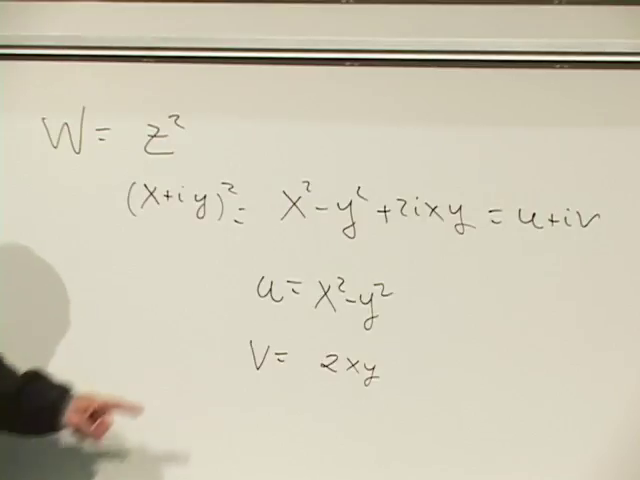
\includegraphics[width=0.68\textwidth]{lecture_08_figure_03.png}
  \caption{Смешанные производные сокращаются, оставляя уравнение Лапласа для одной компоненты аналитического отображения.}
  \lectureframe{00:23:09}
  \label{fig:l08-harmonic-board}
\end{figure}

Существует и полезная векторная интерпретация. Если
\(\mathbf F=(u,-v)\), то два уравнения Коши--Римана, с точностью до выбранного соглашения об ориентации, утверждают, что и дивергенция, и двумерный ротор \(\mathbf F\) равны нулю. Это и есть обещанное возвращение к электростатике.

\subsection{Почему углы сохраняются}

Запишем два малых комплексных смещения в полярной форме:
\begin{equation}
  \delta z=\rho e^{i\theta},
  \qquad
  \Delta z=\rho'e^{i\theta'}.
\end{equation}
Их отношение имеет фазу \(\theta-\theta'\), то есть в точности угол между ними.
При аналитическом отображении,
\begin{equation}
  \frac{\delta w}{\delta z}
  =\frac{\Delta w}{\Delta z}
  =w'(z),
\end{equation}
поскольку производная не зависит от направления. Переставляя члены, получаем
\begin{equation}
  \frac{\Delta z}{\delta z}
  =\frac{\Delta w}{\delta w}.
  \label{eq:l08-angle-ratio}
\end{equation}
У обеих частей одна и та же фаза, поэтому угол между исходными интервалами равен углу между их образами.

\begin{figure}[H]
  \centering
  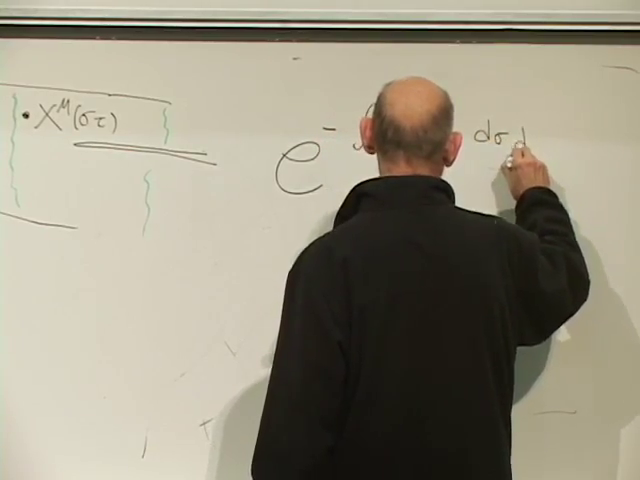
\includegraphics[width=0.70\textwidth]{lecture_08_figure_04.png}
  \medskip

  \begin{tikzpicture}[x=0.9cm,y=0.9cm,>=Latex]
    \begin{scope}
      \draw[->] (-0.2,0) -- (2.3,0);
      \draw[->] (0,-0.2) -- (0,2.1);
      \draw[very thick,blue!65!black,->] (0,0) -- (1.85,0.45)
        node[right] {\(\delta z\)};
      \draw[very thick,orange!75!black,->] (0,0) -- (0.72,1.65)
        node[above] {\(\Delta z\)};
      \draw (0.58,0.14) arc[start angle=14,end angle=66,radius=0.60];
      \node at (1.0,-0.55) {\(z\)-plane};
    \end{scope}
    \draw[->,thick] (3.0,0.9) -- (4.2,0.9)
      node[midway,above] {\(w(z)\)};
    \begin{scope}[xshift=5.0cm]
      \draw[->] (-0.2,0) -- (2.3,0);
      \draw[->] (0,-0.2) -- (0,2.1);
      \draw[very thick,blue!65!black,->] (0,0) -- (1.65,0.70)
        node[right] {\(\delta w\)};
      \draw[very thick,orange!75!black,->] (0,0) -- (0.48,1.62)
        node[above] {\(\Delta w\)};
      \draw (0.54,0.23) arc[start angle=23,end angle=74,radius=0.59];
      \node at (1.0,-0.55) {\(w\)-plane};
    \end{scope}
  \end{tikzpicture}
  \caption{Доказательство на доске и аккуратная локальная реконструкция. Умножение на \(w'(z)\) поворачивает и масштабирует каждое бесконечно малое направление одинаково, сохраняя угол между ними.}
  \lectureframe{00:34:11}
  \label{fig:l08-angle-proof}
\end{figure}

Этот локальный аргумент предполагает \(w'(z)\neq0\). В критической точке отображение может перестать быть локально взаимно однозначным, и тогда геометрию нужно рассматривать отдельно. Вне таких точек аналитические отображения и сохраняющие ориентацию конформные отображения локально являются одними и теми же объектами.

\section{Примеры, тренирующие глаз}

\subsection{Возведение в квадрат и комплексное сопряжение}

Для \(w=z^2\),
\begin{equation}
  (x+iy)^2=x^2-y^2+2ixy=u+iv,
\end{equation}
так что
\begin{equation}
  u=x^2-y^2,
  \qquad
  v=2xy.
  \label{eq:l08-z-squared-components}
\end{equation}
Вторые производные \(u\) равны \(2\) и \(-2\); соответствующие производные \(v\) по отдельности обращаются в нуль. Обе функции гармоничны, и прямое дифференцирование также проверяет уравнения Коши--Римана.

\begin{figure}[H]
  \centering
  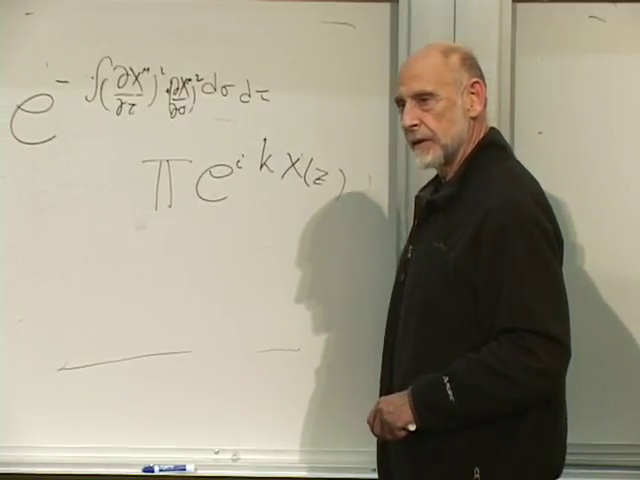
\includegraphics[width=0.72\textwidth]{lecture_08_figure_05.png}
  \caption{Отображение возведения в квадрат, разложенное на его действительную и мнимую гармонические компоненты.}
  \lectureframe{00:36:45}
  \label{fig:l08-z-square-board}
\end{figure}

\begin{classroomqa}
\audiencequestion{Даёт ли \(1/z\) неаналитический пример?
\lecturetimestamp{00:37:49}}
\lecturerresponse{Только в одной точке. Эта функция аналитична всюду, где \(z\neq0\), и имеет полюс в начале координат. Чтобы увидеть отображение, которое всюду не проходит проверку Коши--Римана, лучше взять комплексное сопряжение.}
\end{classroomqa}

Напротив,
\begin{equation}
  w=\bar z=x-iy
  \qquad\Longrightarrow\qquad
  u=x,\quad v=-y
\end{equation}
обращает ориентацию. Его производные не удовлетворяют первому уравнению Коши--Римана из-за знака, так что оно не аналитично как функция \(z\).

\begin{figure}[H]
  \centering
  \includegraphics[width=0.62\textwidth]{lecture_08_figure_06.png}
  \caption{Комплексное сопряжение даёт намеренно неаналитический контрпример.}
  \lectureframe{00:38:38}
  \label{fig:l08-conjugate-board}
\end{figure}

\subsection{Экспонента и её обратная функция}

\begin{classroomqa}
\audiencequestion{Если \(e^z\) аналитична, почему её обратная функция \(\log z\) тоже должна быть аналитичной? \lecturetimestamp{00:40:38}}
\lecturerresponse{Там, где обратная функция существует и \(w'(z)\neq0\), её производная равна \(1/w'(z)\). Поэтому независимость от направления сохраняется. Глобально логарифм многозначен, так что выбирают ветвь и исключают её точку ветвления и разрез. Локальное конформное утверждение остаётся верным на этой выбранной области.}
\end{classroomqa}

Формула Эйлера даёт
\begin{equation}
  w=e^z=e^{x+iy}
  =e^x(\cos y+i\sin y),
\end{equation}
следовательно
\begin{equation}
  u=e^x\cos y,
  \qquad
  v=e^x\sin y.
  \label{eq:l08-exponential-components}
\end{equation}
Например,
\(\partial_xu=e^x\cos y=\partial_yv\), и второе уравнение Коши--Римана получается столь же непосредственно.

\begin{figure}[H]
  \centering
  \includegraphics[width=0.68\textwidth]{lecture_08_figure_07.png}
  \caption{Действительная и мнимая компоненты экспоненциального отображения.}
  \lectureframe{00:42:23}
  \label{fig:l08-exponential-board}
\end{figure}

\section{Полуплоскость, полоса, цилиндр и диск}

\subsection{Логарифм превращает радиус во время}

Возьмём правую полуплоскость, где
\(-\pi/2<\theta<\pi/2\), и запишем
\begin{equation}
  z=re^{i\theta},
  \qquad
  w=\log z=\log r+i\theta.
  \label{eq:l08-log-map}
\end{equation}
Полуплоскость отображается в бесконечную полосу
\begin{equation}
  -\frac{\pi}{2}<\operatorname{Im}w<\frac{\pi}{2}.
\end{equation}
Лучи при фиксированном \(\theta\) переходят в горизонтальные прямые, тогда как полуокружности при фиксированном \(r\) переходят в вертикальные прямые. Начало координат переходит в
\(\operatorname{Re}w=-\infty\), а \(r=\infty\) — в
\(\operatorname{Re}w=+\infty\).

\begin{figure}[H]
  \centering
  \includegraphics[width=0.75\textwidth]{lecture_08_figure_08.png}
  \caption{Логарифм переводит правую полуплоскость в бесконечную полосу: полярные лучи и полуокружности становятся ортогональной прямоугольной сеткой.}
  \lectureframe{00:47:48}
  \label{fig:l08-log-strip-board}
\end{figure}

Полоса является стандартной мировой поверхностью открытой струны. Её ограниченная координата служит параметром вдоль струны, а трансляция вдоль неограниченного направления есть время мировой поверхности. При обратном экспоненциальном отображении перенос по времени становится дилатацией \(z\mapsto e^a z\). Таким образом, одна и та же симметрия выглядит как трансляция на полосе и как однородное растяжение на полуплоскости.

\begin{classroomqa}
\audiencequestion{Куда переходит конкретное значение, например \(r=1\), и остаются ли координаты на полосе полярными? \lecturetimestamp{00:50:58}}
\lecturerresponse{Окружность фиксированного радиуса переходит в вертикальную прямую при \(\operatorname{Re}w=\log r\); в частности, \(r=1\) отображается в центральную линию \(\operatorname{Re}w=0\). Полярные координаты описывают плоскость \(z\). На плоскости \(w\) используются обычные прямоугольные координаты \((\log r,\theta)\).}
\end{classroomqa}

Если всю плоскость с выколотой точкой отобразить при помощи \(\log z\), угловая координата имеет период \(2\pi\). Поэтому у получающейся полосы верхний и нижний края отождествляются: это бесконечный цилиндр. Полуплоскость с границей описывает мировую поверхность открытой струны; вся плоскость без границы и с периодическим углом описывает цилиндр замкнутой струны.

\begin{figure}[H]
  \centering
  \includegraphics[width=0.75\textwidth]{lecture_08_figure_09.png}
  \caption{Представление через полуплоскость и полосу, а также периодическое отождествление, превращающее всю плоскость с выколотой точкой в цилиндр замкнутой струны.}
  \lectureframe{00:54:23}
  \label{fig:l08-open-closed-board}
\end{figure}

\subsection{Отображение Кэли на единичный диск}

Линейно-дробное, или преобразование Мёбиуса, отображает правую полуплоскость на единичный диск:
\begin{equation}
  w=\frac{z-1}{z+1}.
  \label{eq:l08-cayley}
\end{equation}
Оно переводит \(z=0\) в \(-1\), \(z=\infty\) в \(+1\), а мнимую ось — в \(|w|=1\). Если \(z=ir\),
\begin{equation}
  \left|\frac{ir-1}{ir+1}\right|=1.
\end{equation}
Точки с \(\operatorname{Re}z>0\) лежат внутри окружности; левая полуплоскость отображается вне её.
\editorialnote{Во время вывода на доске записывается обратное выражение \((z+1)/(z-1)\), тогда как описывается образ внутри диска. Это обратное выражение имеет ту же границу в виде единичной окружности, но отображает правую полуплоскость во внешнюю область. Формула \eqref{eq:l08-cayley} соответствует соглашению для внутренности диска, согласующемуся с описанной геометрией.}

\begin{figure}[H]
  \centering
  \includegraphics[width=0.72\textwidth]{lecture_08_figure_10.png}
  \caption{Линейно-дробное построение границы единичной окружности. Обратная конвенция, видимая на доске, меняет местами внутренность и внешнюю область.}
  \lectureframe{00:58:38}
  \label{fig:l08-cayley-board}
\end{figure}

Преобразования Мёбиуса переводят обобщённое семейство окружностей и прямых в окружности и прямые. Поэтому радиальная и круговая сетка на полуплоскости превращается в две ортогональные семьи дуг в диске. Прямолинейный диаметр — это просто предельный случай окружности, центр которой ушёл в бесконечность.

\begin{classroomqa}
\audiencequestion{Нарисованные внутри диска дуги действительно являются дугами окружностей?
\lecturetimestamp{01:00:55}}
\lecturerresponse{Да. Их центры находятся в разных местах, часто вне видимого диска. Диаметр — это предел того же семейства при бесконечном радиусе.}
\end{classroomqa}

\begin{classroomqa}
\audiencequestion{Означает ли рисунок диска, что это сфера, и куда девается другая полуплоскость? \lecturetimestamp{01:01:21}}
\lecturerresponse{Изображение здесь — это плоский диск, а не сфера. Правая полуплоскость отображается внутрь его границы, а левая полуплоскость — наружу. Если добавить точку на бесконечности ко всей комплексной плоскости, эту расширенную плоскость можно представить в виде сферы с помощью стереографической проекции; это уже другое глобальное утверждение.}
\end{classroomqa}

\begin{classroomqa}
\audiencequestion{Какие кривые в диске соответствуют исходным радиальным лучам и полуокружностям постоянного радиуса? \lecturetimestamp{01:02:59}}
\lecturerresponse{Положительная вещественная ось становится диаметром, соединяющим \(-1\) и \(+1\). Другие лучи переходят в дуги окружностей, соединяющие те же граничные точки. Полуокружности фиксированного радиуса переходят в ортогональное семейство, которое начинается и заканчивается на единичной окружности.}
\end{classroomqa}

\begin{figure}[H]
  \centering
  \includegraphics[width=0.72\textwidth]{lecture_08_figure_11.png}
  \caption{Прямые и полуокружности в полуплоскости переходят в ортогональные семейства окружностей и прямых в диске.}
  \lectureframe{01:03:48}
  \label{fig:l08-circle-grid-board}
\end{figure}

\section{Мировая поверхность четырёх струн}

Теперь можно вернуться к рассеянию. Две открытые струны входят, сливаются в одну струну, распространяются в течение произвольного промежутка и расщепляются на две выходящие струны. В координатах полосы мировая поверхность выглядит как длинная лента, надрезанная с каждого конца---картинка «спортивного бинта». Промежуточное время жизни заранее не выбирается. Оно является одной из историй, по которым интегрируется амплитуда.

Пусть \((\sigma,\tau)\) — координаты на мировой поверхности, и пусть
\begin{equation}
  X^\mu=X^\mu(\sigma,\tau)
  \label{eq:l08-embedding}
\end{equation}
задаёт её положение в пространстве-времени. Обозначения \(\sigma,\tau\) относятся к двумерной параметрической поверхности; индекс \(\mu\) нумерует координаты пространства-времени. В бозонной теории \(\mu=0,\ldots,25\); в случае суперструны пространственно-временных координат десять.

После поворота Вика свободные поля вложения имеют евклидово действие
\begin{equation}
  S_E[X]
  =\frac{1}{4\pi\alpha'}\int_\Sigma d\sigma\,d\tau\,
  \left[
    \partial_\tau X^\mu\partial_\tau X_\mu
    +\partial_\sigma X^\mu\partial_\sigma X_\mu
  \right].
  \label{eq:l08-euclidean-action}
\end{equation}
Соответствующий функциональный интеграл суммирует по всем вложениям выбранной мировой поверхности в пространство-время:
\begin{equation}
  \int\mathcal D X\,e^{-S_E[X]}.
  \label{eq:l08-bare-worldsheet-integral}
\end{equation}

\begin{figure}[H]
  \centering
  \includegraphics[width=0.74\textwidth]{lecture_08_figure_12.png}
  \caption{Полный положительный евклидов вес мировой поверхности. Два члена с производными суммируются по всем пространственно-временным компонентам.}
  \lectureframe{01:11:34}
  \label{fig:l08-action-board}
\end{figure}

Надрезанная полоса имеет одну связную границу. Поэтому конформная свобода позволяет представить её в виде диска. Четыре удалённых конца полос переходят в четыре отмеченные точки на границе. Деформация отмеченных точек меняет кажущееся расстояние между слиянием и расщеплением в координатах полосы, но не меняет ни саму поверхность, ни физику.

\begin{figure}[H]
  \centering
  \includegraphics[width=0.76\textwidth]{lecture_08_figure_13.png}
  \caption{Мировая поверхность надрезанной полосы и её представление в виде диска с граничными точками для внешних струн.}
  \lectureframe{01:15:18}
  \label{fig:l08-bandage-disc-board}
\end{figure}

Подробные линии сетки, используемые для изображения этого конформного отображения, не несут физического содержания. Существенны топология, граница и отмеченные внешние точки. Одну и ту же мировую поверхность можно растянуть в разные канальные представления, не вводя нового взаимодействия.

\section{Внешние состояния как граничные вставки}

Сам интеграл \eqref{eq:l08-bare-worldsheet-integral} ещё не указывает, какие импульсы входят и выходят. Для скалярного состояния открытой струны с импульсом \(k_i^\mu\) вставим на границе вершинный оператор
\begin{equation}
  V_i(z_i)=e^{\,i k_i\cdot X(z_i)},
  \qquad
  k_i\cdot X=k_{i\mu}X^\mu.
  \label{eq:l08-vertex}
\end{equation}
Точка \(z_i\) — это положение на границе мировой поверхности. Она не является ни координатой пространства-времени, ни направлением импульса.

\begin{figure}[H]
  \centering
  \includegraphics[width=0.72\textwidth]{lecture_08_figure_14.png}
  \caption{Евклидов вес в объёме и произведение граничных импульсных вставок показаны как отдельные множители.}
  \lectureframe{01:18:58}
  \label{fig:l08-vertex-board}
\end{figure}

Для \(n\) внешних открытых струн схематическое предписание имеет вид
\begin{equation}
  \begin{aligned}
    \mathcal A_n(k_1,\ldots,k_n)
    &=\int_{\mathcal M_{0,n}^{\partial}}\!d\mu(z_i)
      \int\mathcal D X\\
    &\quad\times e^{-S_E[X]}
      \prod_{i=1}^{n}e^{\,i k_i\cdot X(z_i)}.
  \end{aligned}
  \label{eq:l08-open-string-prescription}
\end{equation}
Функциональный интеграл берётся по вложениям \(X^\mu\). Конечномерный интеграл берётся по неэквивалентным положениям граничных вставок. Факторы поляризации и мера фиксации калибровки на этом этапе опущены, как и в лекции.
\editorialnote{Полная струнная амплитуда после фиксации калибровки также содержит соответствующий вклад духов, зависящие от состояния вершинные факторы, константы связи и нормировку. Формула
\eqref{eq:l08-open-string-prescription} фиксирует зависимость от полей вложения и положений, выведенную в этой лекции.}

\begin{classroomqa}
\audiencequestion{Если внешние импульсы фиксированы, почему по ним интегрируют? \lecturetimestamp{01:20:42}}
\lecturerresponse{Нет. \(k_i\) — фиксированные метки амплитуды рассеяния. Интегрирование ведётся по полям вложения и по точкам мировой поверхности \(z_i\), в которых вставляются эти фиксированные импульсы. Последний интеграл заменяет интеграл по промежуточному времени жизни в представлении через полосу.}
\end{classroomqa}

\begin{classroomqa}
\audiencequestion{Находится ли произведение вершинных множителей внутри функционального интеграла и является ли оно частью действия? \lecturetimestamp{01:21:39}}
\lecturerresponse{Оно умножает \(e^{-S_E}\) внутри функционального интеграла. Эквивалентно можно внести эти множители в экспоненту и рассматривать их как локализованные источниковые члены, добавленные к действию, но по смыслу это вершинные операторы, а не часть свободного действия в объёме.}
\end{classroomqa}

\begin{figure}[H]
  \centering
  \includegraphics[width=0.76\textwidth]{lecture_08_figure_15.png}
  \caption{Функциональный интеграл, записанный с отдельными множителями
  \(e^{ik_i\cdot X(z_i)}\) для каждой внешней частицы по порядку.}
  \lectureframe{01:23:23}
  \label{fig:l08-full-prescription-board}
\end{figure}

\begin{classroomqa}
\audiencequestion{Почему в \(e^{ik\cdot X}\) после поворота Вика на мировой поверхности всё ещё присутствует \(i\)? \lecturetimestamp{01:23:42}}
\lecturerresponse{Поворот меняет время на мировой поверхности и переводит объёмный вес из \(e^{iS}\) в \(e^{-S_E}\). \(i\) в собственной функции импульса — это фаза Фурье, которая маркирует пространственно-временной импульс. У неё другая роль, и она остаётся.}
\end{classroomqa}

\begin{classroomqa}
\audiencequestion{Определяет ли положение \(z_i\) направление вектора импульса? \lecturetimestamp{01:24:19}}
\lecturerresponse{Нет. Направление закодировано в пространственно-временных компонентах \(k_i^\mu\). Точка вставки \(z_i\) указывает, где этот импульс входит в описание на мировом листе; \(X^\mu(z_i)\) входит в число значений поля, по которым ведётся интегрирование в \(\mathcal D X\).}
\end{classroomqa}

\begin{classroomqa}
\audiencequestion{Передают ли нарисованные углы ножек повязки направления физических импульсов? \lecturetimestamp{01:25:07}}
\lecturerresponse{Нет. Повязка — это пространство параметров, а не изображение струны в физическом пространстве-времени. Её ножки можно рисовать горизонтальными, наклонными или конформно изогнутыми. Физические направления задаются компонентами \(k^\mu\), тогда как по \(X^\mu(\sigma,\tau)\) ведётся интегрирование.}
\end{classroomqa}

\section{Гауссов интеграл как электростатика}

Действие \eqref{eq:l08-euclidean-action} квадратично по каждой компоненте \(X^\mu\), а вставки после объединения их экспонент с действием становятся линейными источниками. Поэтому функциональный интеграл является гауссовым. В седловой точке каждая пространственно-временная компонента удовлетворяет уравнению Пуассона схематического вида
\begin{equation}
  \nabla^2 X^\mu(z)
  \propto
  i\alpha'\sum_i k_i^\mu\,\delta(z-z_i),
  \label{eq:l08-electrostatic-source}
\end{equation}
с граничным условием открытой струны на границе диска. Каждое \(X^\mu\) ведёт себя как независимый электростатический потенциал, а каждая компонента импульса \(k_i^\mu\) — как соответствующий заряд, помещённый в \(z_i\).

\begin{figure}[H]
  \centering
  \includegraphics[width=0.76\textwidth]{lecture_08_figure_16.png}
  \caption{Диск с граничными источниками интерпретируется как одна независимая двумерная электростатическая задача для каждой пространственно-временной компоненты.}
  \lectureframe{01:28:58}
  \label{fig:l08-electrostatic-disc-board}
\end{figure}

Решите электростатическую задачу, вычислите её энергию, возведите в экспоненту отрицательную энергию и, наконец, проинтегрируйте по неэквивалентным положениям зарядов. В стандартной нормировке открытой струны коррелятор поля вложения даёт фактор Кобы--Нильсена
\begin{equation}
  \left\langle\prod_i e^{\,ik_i\cdot X(z_i)}\right\rangle
  \propto
  (2\pi)^D\delta^{(D)}\!\left(\sum_i k_i\right)
  \prod_{i<j}|z_i-z_j|^{2\alpha' k_i\cdot k_j}.
  \label{eq:l08-koba-nielsen}
\end{equation}
Дельта-функция выражает сохранение импульса. Произведение содержит попарные электростатические энергии. Для четырёх скалярных граничных вставок, используемых здесь, фиксация трёх положений превращает оставшийся интеграл в эйлеров бета-интеграл, встречавшийся в предыдущих лекциях.

\begin{classroomqa}
\audiencequestion{Имеется двадцать шесть электростатических энергий или только одна?
\lecturetimestamp{01:30:53}}
\lecturerresponse{Для каждой пространственно-временной компоненты имеется по одному независимому потенциалу и полю. Их квадратичные энергии не содержат перекрёстных членов в ортонормированном базисе пространства-мишени, и вклады складываются в одно полное действие до экспоненцирования.}
\end{classroomqa}

\begin{classroomqa}
\audiencequestion{Является ли угловая координата диска физическим углом рассеяния? \lecturetimestamp{01:32:10}}
\lecturerresponse{Нет. Это параметр положения на мировом листе. Соответствующая неэквивалентная комбинация связана с промежуточным интервалом распространения и интегрируется. Физический угол рассеяния закодирован через лоренцевы инварианты, построенные из фиксированных импульсов.}
\end{classroomqa}

\begin{classroomqa}
\audiencequestion{Почему это построение перестаёт работать вне критической размерности? \lecturetimestamp{01:32:35}}
\lecturerresponse{Одни лишь формальные гауссовы интегралы ещё не составляют полного условия согласованности. Фиксация калибровки вводит конформную аномалию, причём вклады материи и духов взаимно сокращаются только в критической размерности: \(D=26\) для бозонной струны и \(D=10\) для суперструны. Без этого сокращения теряется предполагаемая конформная симметрия квантового мирового листа.}
\end{classroomqa}

\begin{classroomqa}
\audiencequestion{Предположили ли мы уже три больших пространственных измерения и компактные дополнительные измерения? \lecturetimestamp{01:33:38}}
\lecturerresponse{Нет. Компактификация ещё не вошла в построение. На этой стадии бозонные координаты по-прежнему пробегают все двадцать шесть направлений пространства-мишени, или десять в случае суперструны. То, как некоторое подмножество может оставаться макроскопически большим, — предмет следующего обсуждения.}
\end{classroomqa}

\begin{classroomqa}
\audiencequestion{Связь с электростатикой состоит просто в том, что координаты удовлетворяют уравнению Лапласа? \lecturetimestamp{01:33:57}}
\lecturerresponse{Именно. Вдали от точек вставки каждое \(X^\mu\) является гармонической функцией; вершинные операторы дают источники в виде дельта-функций. Математически это та же краевая задача, что и для статического двумерного потенциала с точечными зарядами, независимо от того, пользуемся ли мы электростатической терминологией.}
\end{classroomqa}

\subsection{Конформная избыточность и число модулей}

Диск обладает группой конформных автоморфизмов с тремя вещественными параметрами, \(\mathrm{PSL}(2,\mathbb R)\). Поэтому три упорядоченные граничные точки можно зафиксировать в удобных местах. Для четырёх внешних струн остаётся проинтегрировать только четвёртое положение; для \(n\) упорядоченных граничных вставок на уровне дерева имеется
\begin{equation}
  n-3
  \label{eq:l08-n-minus-three}
\end{equation}
вещественных интегралов по положениям.

\begin{classroomqa}
\audiencequestion{Имеются ли вокруг диска четыре независимых угловых положения? \lecturetimestamp{01:34:37}}
\lecturerresponse{Не в физическом смысле. Сначала записывают четыре положения, но конформная симметрия диска позволяет поместить любые три из них где угодно, как удобно. Для амплитуды с двумя входящими и двумя исходящими струнами остаётся только относительное положение четвёртой.}
\end{classroomqa}

\begin{figure}[H]
  \centering
  \includegraphics[width=0.72\textwidth]{lecture_08_figure_17.png}
  \caption{Четыре граничные вставки на диске. Конформная свобода фиксирует любые три, оставляя один четырёхточечный модуль.}
  \lectureframe{01:35:18}
  \label{fig:l08-fix-three-board}
\end{figure}

\begin{classroomqa}
\audiencequestion{Что, если две точки расщепления на рисунке полосы оказываются не на одной высоте? \lecturetimestamp{01:35:24}}
\lecturerresponse{Конформное отображение может убрать это кажущееся несовпадение. Разные рисунки являются координатными представлениями одного и того же модуля. Инвариантным является именно интегрирование по оставшемуся граничному положению, или, что то же, по интервалу распространения.}
\end{classroomqa}

\begin{classroomqa}
\audiencequestion{Для большего числа внешних частиц сколько параметров положения остаётся? \lecturetimestamp{01:36:00}}
\lecturerresponse{Зафиксируйте три точки вставки с помощью конформной симметрии и проинтегрируйте по \(n-3\) остальным параметрам положения. Это и есть подсчёт числа граничных модулей для упорядоченной амплитуды открытой струны на уровне дерева.}
\end{classroomqa}

\begin{classroomqa}
\audiencequestion{Как это связано с М-теорией?
\lecturetimestamp{01:36:37}}
\lecturerresponse{Пока никак. Рассматриваемое здесь построение — это пертурбативное рассеяние открытых струн на мировом листе. Его связь с М-теорией требует более поздних идей о дуальностях и непертурбативных эффектах, поэтому этот вопрос здесь явно откладывается.}
\end{classroomqa}

\begin{classroomqa}
\audiencequestion{Является ли другое вертикальное или перекрещённое изображение полосы другим вычислением? \lecturetimestamp{01:36:49}}
\lecturerresponse{Нет. Можно зафиксировать удобную точку и позволить оставшемуся модулю пробегать весь свой интервал. Изображения полосы и интеграл по граничной точке на диске — это разные разбиения одного и того же интеграла, поэтому все внешние струны можно рассматривать симметрично.}
\end{classroomqa}

\section{Чего это предписание пока не решает}

Формула для диска сразу обобщается на большее число внешних струн: добавьте больше вершинных операторов и проинтегрируйте по их \(n-3\) неэквивалентным граничным положениям. Это точное предписание на уровне дерева для согласованной струнной модели, но пока ещё не реалистическая модель наблюдаемой физики элементарных частиц. Простая бозонная теория имеет неправильную размерность пространства-времени и дополнительные физические недостатки. Суперструны улучшают спектр и понижают критическую размерность до десяти, но шесть пространственных измерений всё ещё необходимо компактфицировать.

\begin{classroomqa}
\audiencequestion{Согласуется ли эта простая модель уже с экспериментами по столкновениям частиц? \lecturetimestamp{01:39:06}}
\lecturerresponse{Нет. Резонансная структура исторически напоминает адронное рассеяние, но двадцатишестимерная бозонная модель не может быть прямым описанием наблюдаемых частиц. Формализм определяет амплитуды рассеяния для этой модели; для соответствия природе требуются реалистический спектр, компактификация, взаимодействия и выбор вакуума.}
\end{classroomqa}

\begin{classroomqa}
\audiencequestion{Сможет ли компактификация уменьшить размеры дополнительных измерений и дать реалистические данные о частицах? \lecturetimestamp{01:41:10}}
\lecturerresponse{Она может уменьшить эффективную макроскопическую размерность и породить спектры частиц и калибровочные группы. Именно здесь возникает и значительная часть подлинной математической трудности. Известно много согласованных компактификаций, и выбор единственной модели наблюдаемых элементарных частиц остаётся нерешённым.}
\end{classroomqa}

В лекции подчёркивается именно это различие, а не предлагается завершённая теория. Струнные построения математически вполне определённы и дали глубокую информацию о гравитации и геометрии, однако сама их множественность является частью физической проблемы.

\begin{classroomqa}
\audiencequestion{Есть ли короткий способ запомнить, почему критическая размерность бозонной струны равна двадцати шести? \lecturetimestamp{01:43:19}}
\lecturerresponse{В более раннем осцилляторном расчёте использовалась регуляризованная сумма нулевой энергии \(1+2+3+\cdots=-1/12\). Вклад поперечных осцилляторов включает двадцать четыре направления, а восстановление двух продольных пространственно-временных координат даёт \(24+2=26\). Это мнемоническое правило для прежнего аргумента согласованности, а не новый вывод здесь.}
\end{classroomqa}

\begin{classroomqa}
\audiencequestion{Квантуются ли сами вставляемые импульсы \(k_i\)?
\lecturetimestamp{01:43:46}}
\lecturerresponse{В некомпактном пространстве-времени их компоненты непрерывны.
Квантуется уровень осциллятора и, следовательно, спектр допустимых значений квадрата массы. В компактных измерениях соответствующие компоненты импульса и намотки могут квантуваться, но это относится к следующему обсуждению.}
\end{classroomqa}